\nwfilename{mainlitprog.nw}\nwbegindocs{0}\section{Introduction}% ===> this file was generated automatically by noweave --- better not edit it




\begin{figure}[H]
\centering
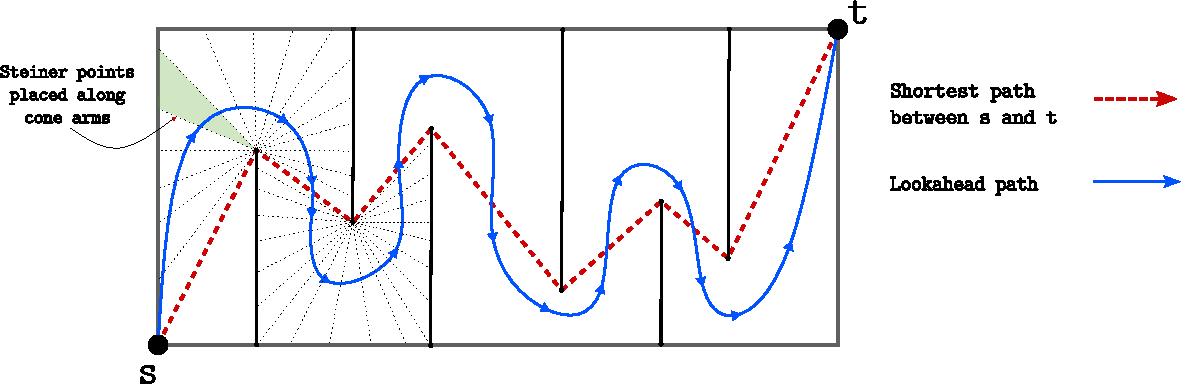
\includegraphics[width=16cm]{miscimages/stalactites-stalagmites.pdf}
\caption{Conical Routing between start $s$ and destination $t$}
\label{fig:conical-routing}
\end{figure}

We report some results on schemes in computing paths with lookahead in the stalactite and stalagmite setting. In a path with lookahead
any point on the path can see a large chunk of the path immediately ahead of it. \footnote{we are using euclidean vision where two points $A$ and $B$ see one another
iff the straight line segment $AB$ is contained in the closure of the free space. } More precisely, given a parameter $l\in \RR^{+}$ we want to compute a shortest 
path between $s$ and $t$ such that point on the computed path satisfies one of either of the two following properties


\begin{itemize}
\item The point can see at least a subpath of length $\geq l$ immediately ahead of it
\item The part of the subpath that the point can see ahead of it contains $t$
\end{itemize}

We will give a set of schemes for doing this in the alternating \textit{stalactites and stalagmites} --- henceforth shortened to ``*ites'' --- such that the shortest path 
between two given points $s$ and $t$ is taut against the tips of the ``*ites''. 



\section{Basic scheme}



%%%%%%%%%%%%%%%%%%%%%%%%%%%%%%%%%%%%%%%%%%%%%%%%%%%%%%%%%%%%%%5
% Description of the rocking line setup and bipartite graph
%%%%%%%%%%%%%%%%%%%%%%%%%%%%%%%%%%%%%%%%%%%%%%%%%%%%%%%%%%%%%
\begin{figure}[H]
\centering
\begin{minipage}[t]{0.45\textwidth}
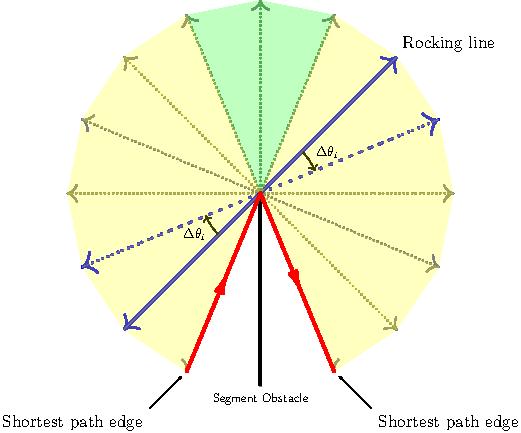
\includegraphics[width=\textwidth]{asy2d/rocking-line.pdf}
\end{minipage}
\begin{minipage}[t]{0.3\textwidth}
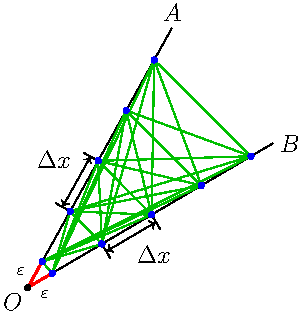
\includegraphics[width=\textwidth]{asy2d/bipartite-cone.pdf}
\end{minipage}
\caption{(Left) A rocking line (blue) creates a sequence of cones of angles 
     $\Delta \theta_i$ between two successive shortest path edges. (Right) Complete bipartite graph (green) between points on two arms of a cone on the Steiner points. 
              Distance between two consecutive Steiner points along each arm is $\Delta x$. $O$ is the tip of the 
      stalactite/stalagmite.}
\label{fig:geomdisc}
\end{figure}






 \begin{itemize}
  \item At each tip $T$ of the *ites, consider the two shortest path edge between $s$ and $t$ incident at that point. Divide the angle between them into 
        yellow and green wedges as shown in the left hand side \autoref{fig:geomdisc}. Each yellow wedge is divided into cones of small angle $\Delta \theta$
        whereas the green wedge is divided into small cones again of size $\Delta \theta$, allowing for one of the cones to have angle $\leq \Delta \theta$

 \item Place Steiner points separated by a small distance $\Delta x$ starting from the obstacle segment tip along each arm of every cone, 
        for as long as the cone arm lies inside free space. Also add the endpoints of the segments as Steiner points of those respective segments. 
       \footnote{computing these is just a simple matter of ray-shooting. }
 \item Draw the complete bipartite graph between the Steiner points of each cone  as shown in \autoref{fig:geomdisc}
 \item Solve the following integer program. 
           

\begin{align}
\min \sum_{e \in E} c_e x_e   &= 2
\end{align}

such that 

\begin{align}
  x_e \in \{0,1\} \\
     \alpha + \beta = \gamma
\end{align}


 \end{itemize}



 This scheme has been implemented in Python 2.7.12 using the Python bindings of CGAL (especially those of its kernel) on a Thinkpad laptop running Linux Mint. 
\nwenddocs{}


